\documentclass[10pt]{beamer}

\input{/Users/daniel/Documents/LaTeX/beamer-style.tex}


\title{Développement d'applications mobiles}
\subtitle{Introduction}
\date{\today}
\author{Daniel Schreurs}
\institute{Haute École de la Province de Liège}
%\titlegraphic{\hfill\includegraphics[height=1.5cm]{logo.eps}}

\begin{document}

\maketitle

\setbeamerfont{subsection in toc}{size=\small}
\begin{frame}[allowframebreaks]{Table des matières}
    \setbeamertemplate{section in toc}[sections numbered]
    \tableofcontents
\end{frame}

\section{Introduction}

\subsection{Comment communiquer ?}
\begin{frame}{\secname : \subsecname}
    \begin{itemize}
        \item Toutes les ressources : sur Moodle;
        \item Une question relative au cours : Forum du cours (sur Moodle);
        \item Une question personnelle : \href{mailto:daniel.schreurs@hepl.be}{daniel.schreurs@hepl.be}.
    \end{itemize}
\end{frame}

\section{Contexte historique}
\subsection{Retour en 2007}
\begin{frame}[fragile,t]{\secname : \subsecname}
    \begin{figure}
        \begin{center}
            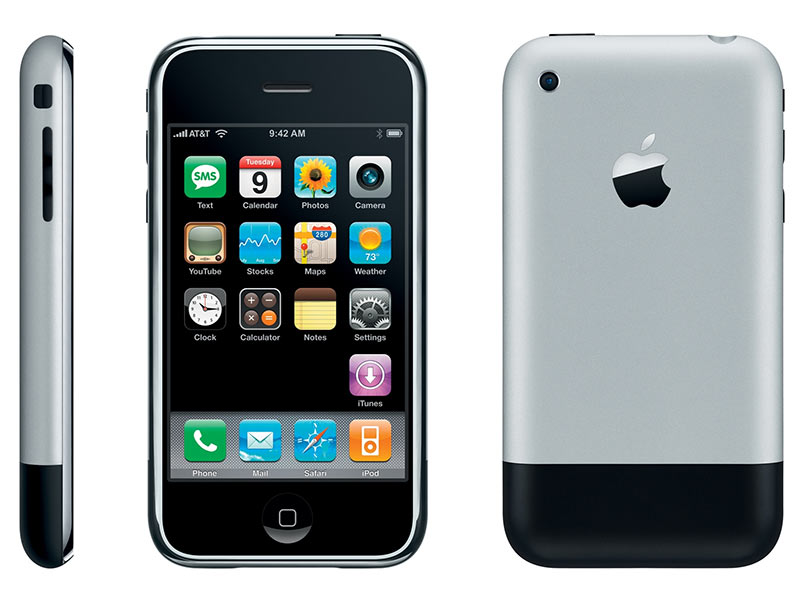
\includegraphics[width=0.5\textwidth]{../assets/img/Originele-iPhone.jpg}
            \caption*{Tout commence en juin 2007 avec l'iPhone.}
            \label{Fig:Originele-iPhone}
        \end{center}
    \end{figure}
\end{frame}

\subsection{Shopping time !}
\begin{frame}[fragile,t]{\secname : \subsecname}
    \begin{figure}
        \begin{center}
            
\includegraphics[width=0.8\textwidth]{../assets/img/android_and_apple.jpg}
            \caption*{L'App Store a ouvert 07/2008 - Android Market 10/2008.}
            \label{Fig:android_and_apple}
        \end{center}
    \end{figure}
\end{frame}

\subsection{La situation}
\begin{frame}[fragile,t]{\secname : \subsecname}
    \begin{itemize}
        \item Développer pour les 2 plateformes;
        \item Si vous avez les moyens de développer une application, vous êtes l'enfant cool du quartier;
        \item Risques et des coûts élevés;
        \item Les coûts explosent car il faut maintenir plusieurs bases de code;
        \item Deux grandes tendances :
              \begin{itemize}
                  \item Natif;
                  \item Sites Web responsives.
              \end{itemize}
    \end{itemize}
\end{frame}

\subsection{L'essor des solutions web}
\begin{frame}[fragile,t]{\secname : \subsecname}
    \begin{itemize}
        \item Moins cher;
        \item Technologies plus matures;
        \item Merci HTML5 et aux WebViews;
        \item Par exemples : \href{https://cordova.apache.org}{Cordova};
        \item Ces applications avaient souvent du mal à reproduire l'aspect et la convivialité des applications natives.
    \end{itemize}
\end{frame}

\subsection{Des solutions hybrides}
\begin{frame}[fragile,t]{\secname : \subsecname}
    \begin{itemize}
        \item En 2015 Facebook dévoile React Native;
        \item Une solution hybride :
              \begin{itemize}
                  \item Même logique métier que celle du web ( JavaScript);
                  \item Utiliser un WebView, mais un système de rendu natif.
              \end{itemize}
        \item Le succès est énorme;
        \item Mais des améliorations sont possibles (voir nécessaire).
    \end{itemize}
\end{frame}


\section{Flutter}
\subsection{Flutter, c'est quoi ?}
\begin{frame}[fragile,t]{\secname : \subsecname}
    \begin{itemize}
        \item A software development toolkit, de Google;
        \item Permet de construire des applications multiplateformes;
        \item Des paquets, plug-ins et beaucoup de widgets;
        \item Flutter n'est pas un langage;
        \item Flutter utilise \href{https://dart.dev}{Dart} comme langage de programmation.
    \end{itemize}
\end{frame}

\subsection{Quelques forces}
\begin{frame}[fragile,t]{\secname : \subsecname}
    \begin{itemize}
        \item Flutter permet de compiler pour le Web, Android et IOS;
        \item Flutter est open source;
        \item Flutter utilise un langage récent \href{https://dart.dev}{Dart};
        \item Flutter permet le rechargement à chaud (\href{https://flutter.dev/docs/development/tools/hot-reload}{hot reload});
        \item Flutter \href{https://flutter.dev/docs/development/ui/widgets/material}{supporte nativement} le \href{https://material.io/design/guidelines-overview}{Material Design} de Google;
        \item Flutter permet de programmer des animations et transitions personnelles ou déjà existantes;
        \item Flutter permet le databinding;
        \item Les concepts de flutter sont proches de \href{https://developer.apple.com/xcode/swiftui/}{SwiftUI} et \href{https://developer.android.com/jetpack/compose}{Jetpack Compose}.
        \item Flutter permet de faire des applications accessibles.
    \end{itemize}
\end{frame}

\subsection{Quelques faiblesses}
\begin{frame}[fragile,t]{\secname : \subsecname}
    \begin{itemize}
        \item Ce n'est pas du développement natif;
        \item N'est pas adapté pour des jeux et/ou applications audios;
        \item N'est pas adapté pour des besoins très spécifiques de l'environnement Apple;
        \item Ne supporte pas watchOS, tvOS etc.;
        \item C'est un pari sur l'avenir, la technologie est très récente.
    \end{itemize}
\end{frame}

\subsection{Quelques Exemples}
\begin{frame}[fragile,t]{\secname : \subsecname}
    \begin{figure}[H]
        \begin{center}
            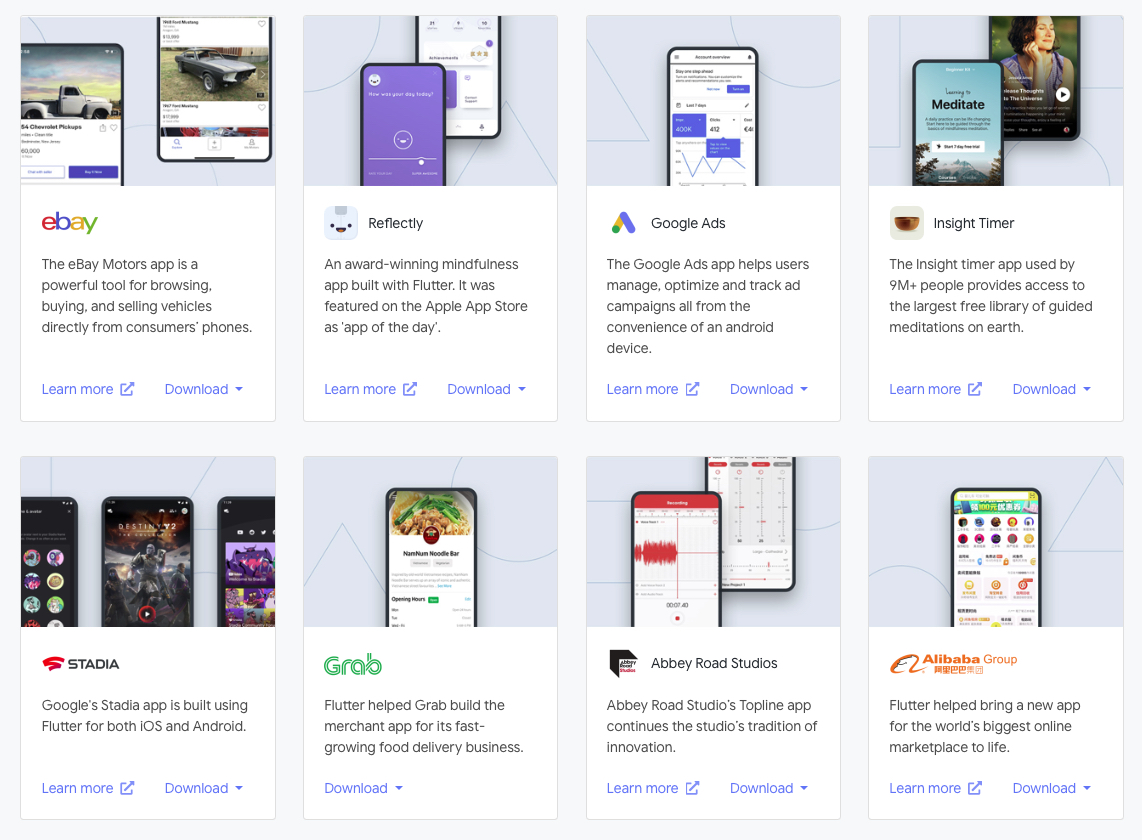
\includegraphics[width=0.7\textwidth]{../assets/img/exemples.jpg}
            \caption*{Quelques exemples parmi d'autres : \href{https://flutter.dev/showcase}{Apps take flight with Flutter}}
            \label{Fig:exemples}
        \end{center}
    \end{figure}
\end{frame}

\begin{frame}[fragile,t]{\secname : \subsecname}
    \begin{figure}[H]
        \begin{center}
            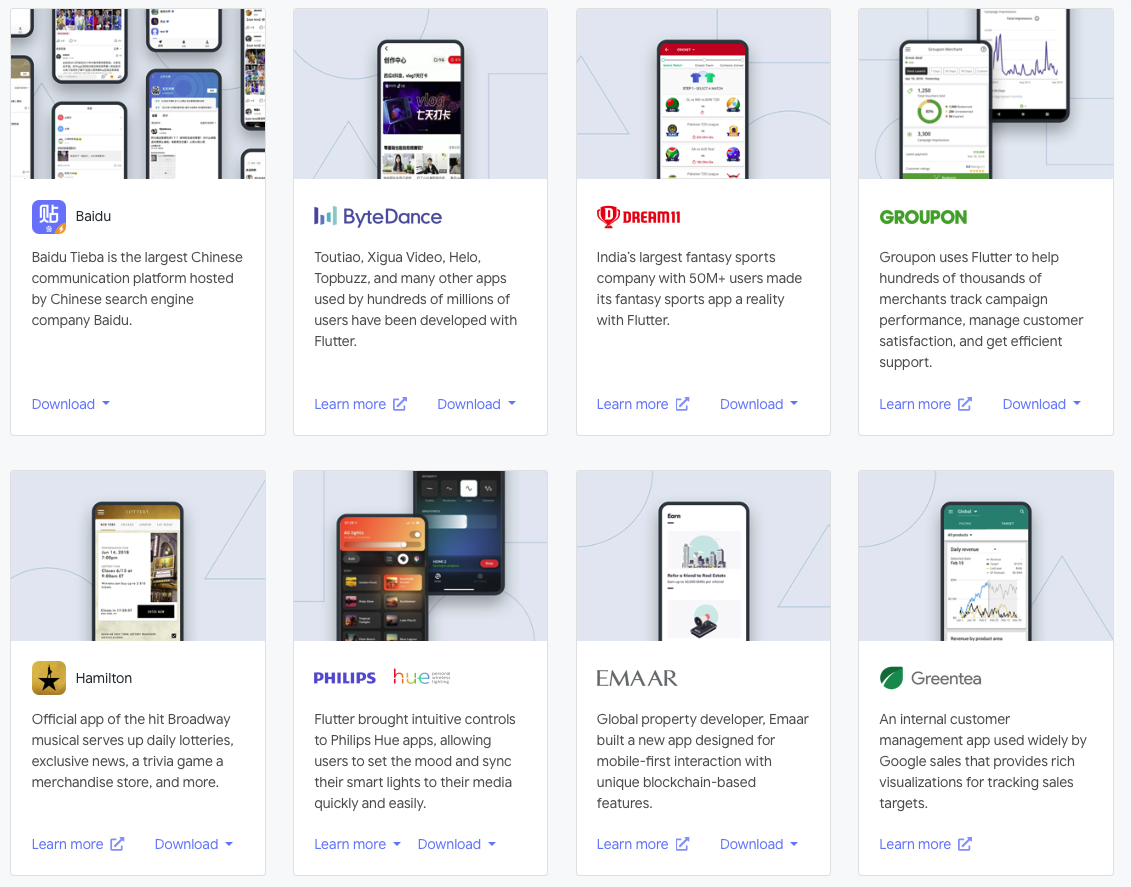
\includegraphics[width=0.7\textwidth]{../assets/img/exemples2.jpg}
            \caption*{Quelques exemples parmi d'autres : \href{https://flutter.dev/showcase}{Apps take flight with Flutter}}
        \end{center}
    \end{figure}
\end{frame}

\section{Architecture}

\subsection{Flutter}
\begin{frame}[fragile,t]{\secname : \subsecname}
    \begin{figure}[H]
        \begin{center}
            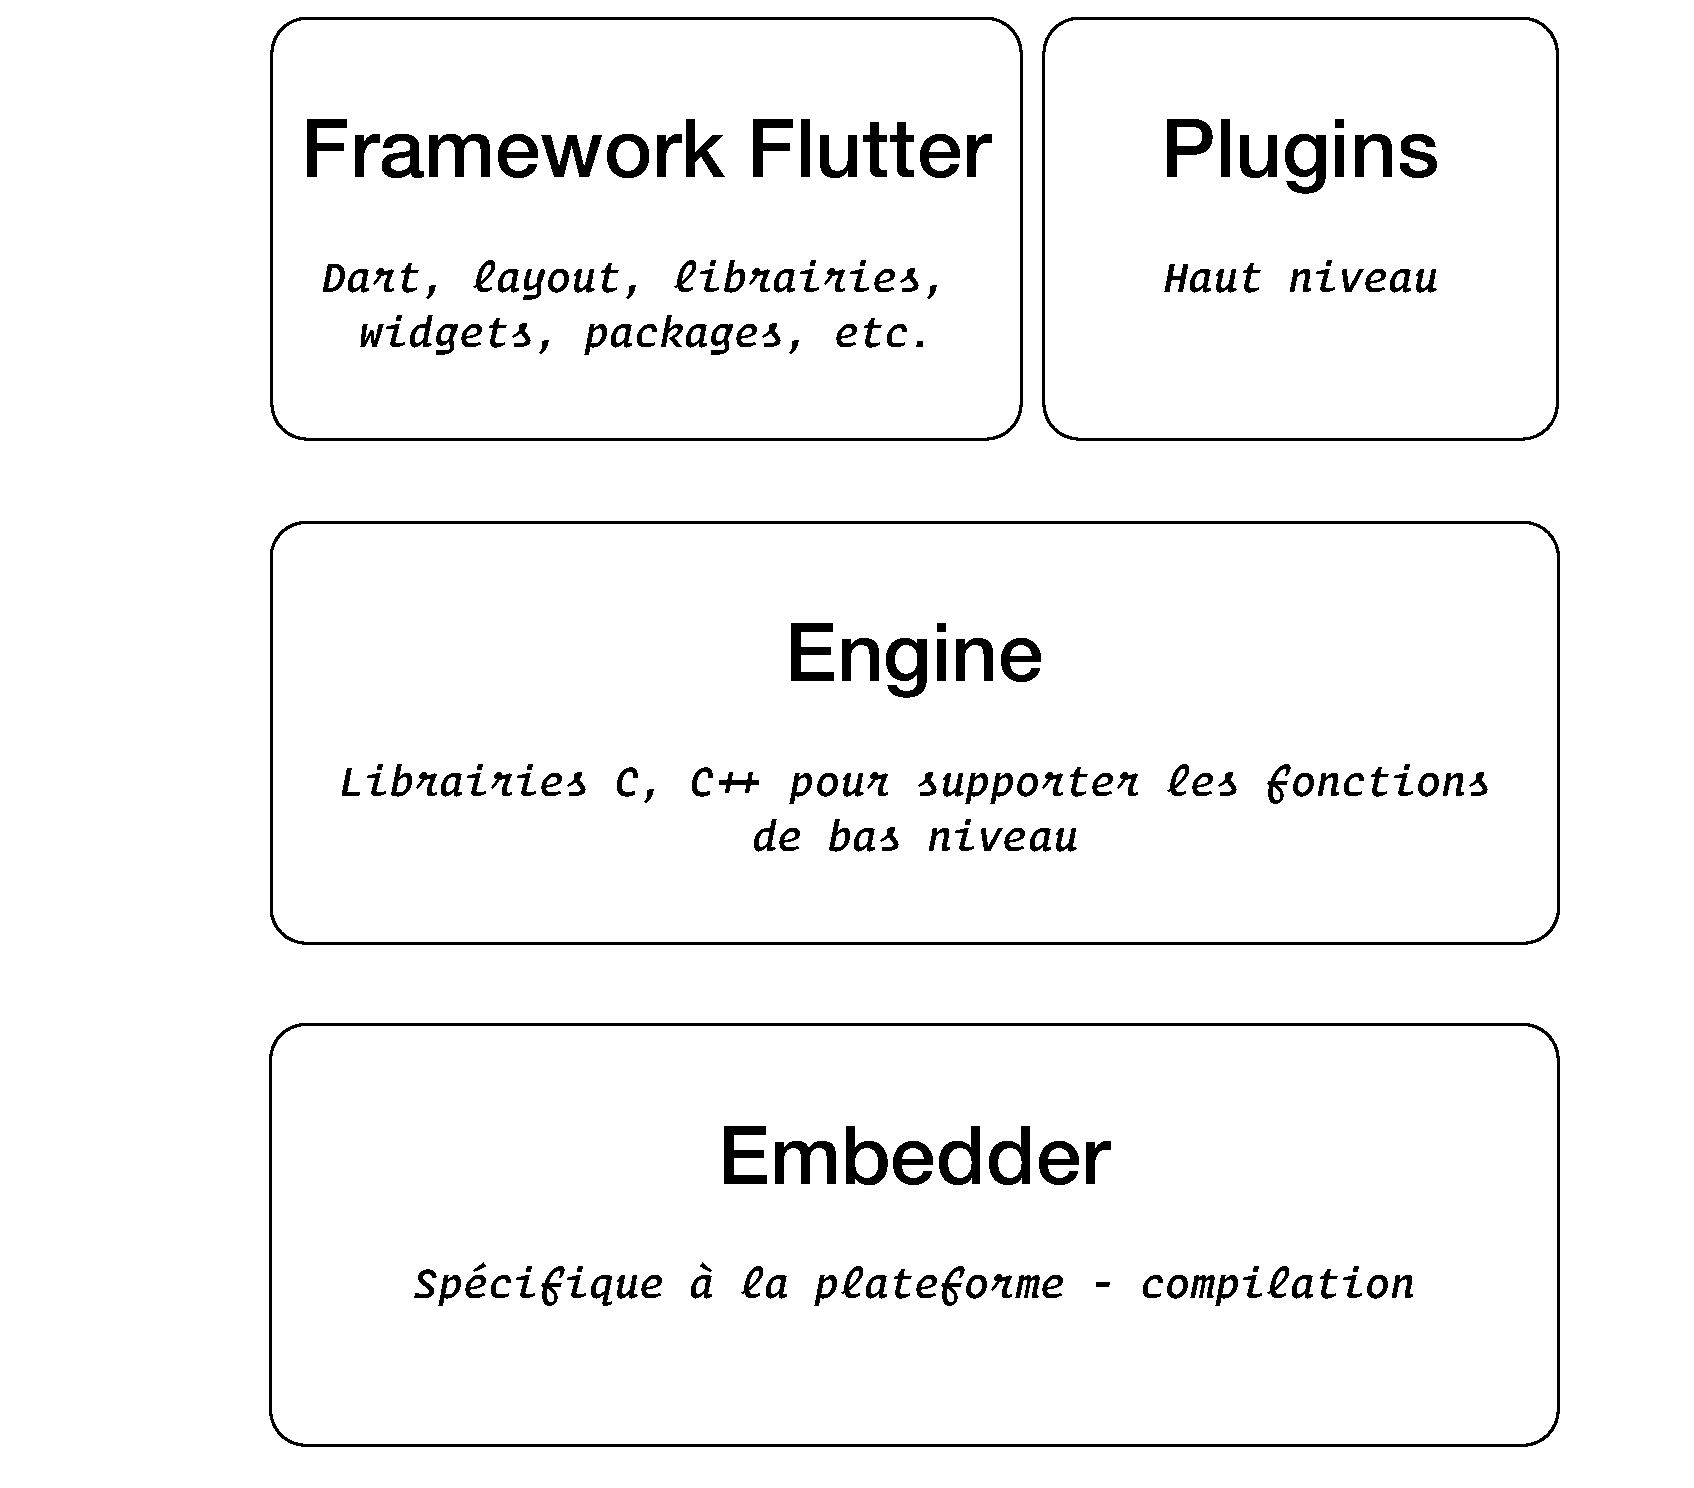
\includegraphics[width=0.5\textwidth]{../assets/img/architecture-flutter.eps}
            \caption*{Architecture Flutter}
            \label{Fig:architecture-flutter}
        \end{center}
    \end{figure}
\end{frame}

\subsubsection{Framework Flutter}
\begin{frame}[fragile,t]{\secname : \subsecname}
    \begin{itemize}
        \item Le \textbf{Framework Flutter} est écrit en Dart;
        \item Il contient des bibliothèques de haut niveau avec notamment :
              \begin{itemize}
                  \item Les thèmes;
                  \item Les widgets;
                  \item La mise en page;
                  \item Les animations.
              \end{itemize}
    \end{itemize}
\end{frame}
\subsubsection{Plug-ins}
\begin{frame}[fragile,t]{\secname : \subsecname}
    \begin{itemize}
        \item Les \textbf{Plugins} isolent des fonctionnalités de haut niveau :
              \begin{itemize}
                  \item La sérialisation JSON;
                  \item La géolocalisation;
                  \item L'accès aux caméras;
                  \item Les paiements in-app, etc.
              \end{itemize}
    \end{itemize}
\end{frame}

\subsubsection{Engine}
\begin{frame}[fragile,t]{\secname : \subsecname}
    \begin{itemize}
        \item La couche \textbf{Engine} contient les bibliothèques C++. Elle gère :
              \begin{itemize}
                  \item Les graphiques;
                  \item La mise en page du texte;
                  \item L'accessibilité;
                  \item L'architecture des plugins et le moteur d'exécution Dart.
              \end{itemize}
    \end{itemize}
\end{frame}

\subsubsection{Engine}
\begin{frame}[fragile,t]{\secname : \subsecname}
    \begin{itemize}
        \item L'\textbf{Embedder} est différent pour chaque plateforme cible. Il gère :
              \begin{itemize}
                  \item L'\textit{empaquetage} du code comme une application autonome.
              \end{itemize}
    \end{itemize}
\end{frame}

\begin{frame}[fragile,t]{\secname : \subsecname}
    \metroset{block=fill}
    \begin{block}{Remarque}
        Chacune des couches est encore une fois décomposée en plusieurs sous-couches.
    \end{block}
\end{frame}

\subsection{Découpe de la couche Framework}
\begin{frame}[fragile,t]{\secname : \subsecname}
    \begin{figure}[H]
        \begin{center}
            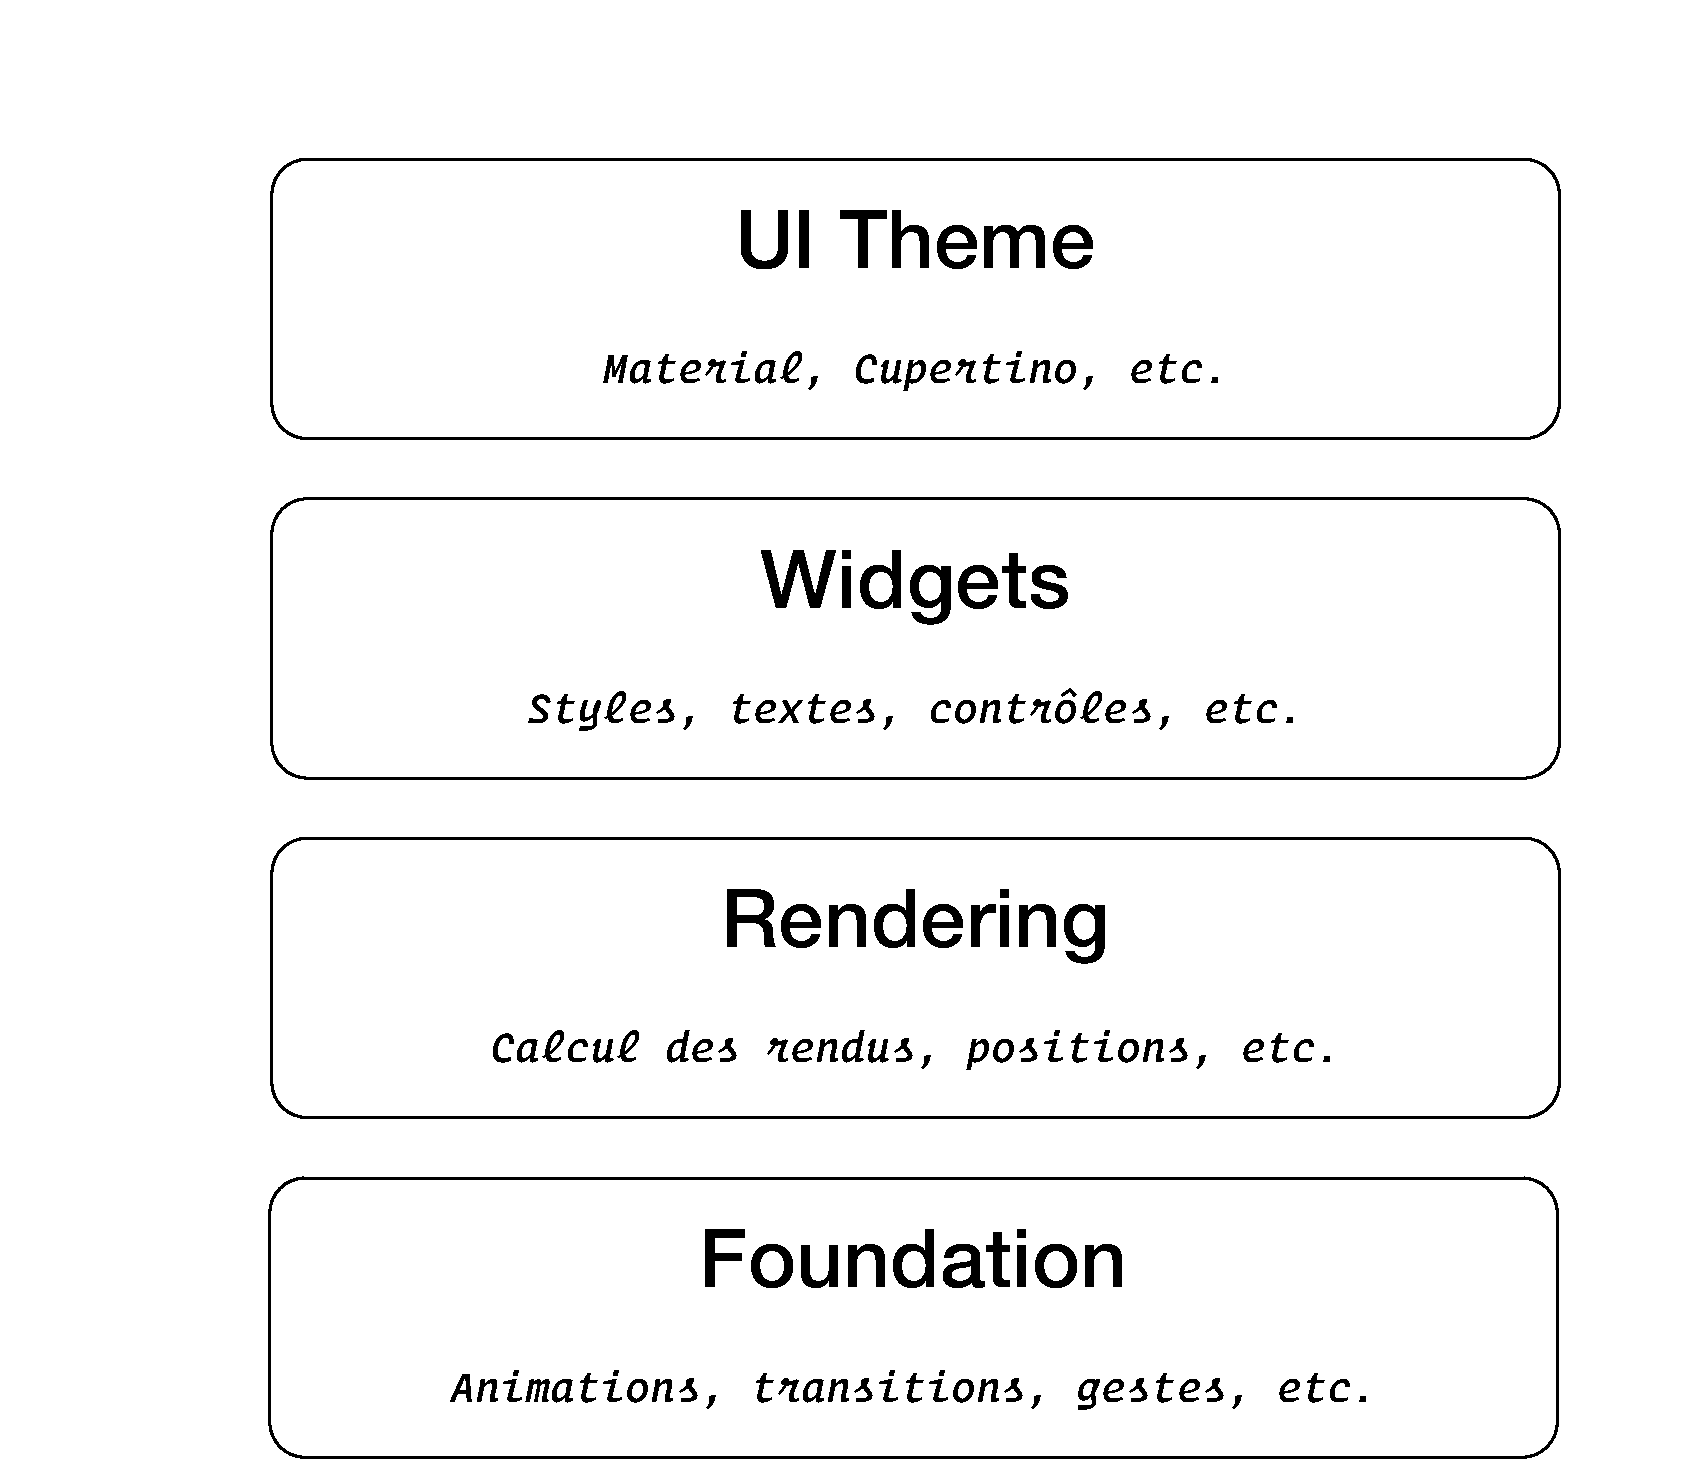
\includegraphics[width=0.5\textwidth]{../assets/img/architecture-framework.eps}
            \caption*{Architecture du framework Flutter}
            \label{Fig:architecture-framework}
        \end{center}
    \end{figure}
\end{frame}

\begin{frame}[fragile]{What’s new in Flutter 3 ?}
    \begin{quote}
        \href{https://medium.com/flutter/whats-new-in-flutter-3-8c74a5bc32d0}{What’s new in Flutter 3?}
    \end{quote}
\end{frame}


\end{document}